\documentclass[a4paper, 11pt, oneside]{article} % A4 paper size, default 11pt font size and oneside for equal margins

\newcommand{\plogo}{\fbox{$\mathcal{PL}$}} % Generic dummy publisher logo

\usepackage[utf8]{inputenc} % Required for inputting international characters
\usepackage[T1]{fontenc} % Output font encoding for international characters
\usepackage{fouriernc} % Use the New Century Schoolbook font
\usepackage{graphicx}
\usepackage{amsmath}
\usepackage{float}
\usepackage[export]{adjustbox}
\usepackage[hidelinks]{hyperref}

\begin{document}

\begin{titlepage} % Suppresses headers and footers on the title page

	\centering % Centre everything on the title page
	
	\scshape % Use small caps for all text on the title page
	
	\vspace*{\baselineskip} % White space at the top of the page
	
	%------------------------------------------------
	%	Title
	%------------------------------------------------
	
	\rule{\textwidth}{1.6pt}\vspace*{-\baselineskip}\vspace*{2pt} % Thick horizontal rule
	\rule{\textwidth}{0.4pt} % Thin horizontal rule
	
	\vspace{0.75\baselineskip} % Whitespace above the title
	
	{\LARGE CSE 406\\ Computer Security Sessional\\ Offline Report\\ Cross Site Scripting} % Title
	
	\vspace{0.75\baselineskip} % Whitespace below the title
	
	\rule{\textwidth}{0.4pt}\vspace*{-\baselineskip}\vspace{3.2pt} % Thin horizontal rule
	\rule{\textwidth}{1.6pt} % Thick horizontal rule
	
	\vspace{\baselineskip} % Whitespace after the title block
	
	%------------------------------------------------
	%	Subtitle
	%------------------------------------------------
	

 {DEPARTMENT OF COMPUTER SCIENCE AND ENGINEERING \\ \vspace{0.75\baselineskip} BANGLADESH UNIVERSITY OF \\ \vspace{0.5\baselineskip} ENGINEERING AND TECHNOLOGY}% Subtitle or further description
	
	\vspace*{2\baselineskip} % Whitespace under the subtitle
	
	%------------------------------------------------
	%	Editor(s)
	%------------------------------------------------
	
	LAB SUBSECTION: A2 \\
 \vspace{0.75\baselineskip}
        SUBMITTED BY: 1905041 \\
        \vspace{0.75\baselineskip}
   
	\vspace{1\baselineskip} % Whitespace below the editor list
	
	\textit{SUBMITTED ON: 13/02/2024} % Editor affiliation
	

\end{titlepage}

\tableofcontents
\newpage

\section{Task 1: Adding User as Samy's Friend}
\subsection{Method}
For this task, first the request for adding a user as a friend was examined. The URL(\texttt{http://www.seed-server.com/action/friends/add?friend=59}), the request type(GET) and the query parameters(\texttt{friend, \_\_elgg\_token, \_\_elgg\_ts}) was noted. A script was written that gets these values from the \texttt{elgg.session.user} and the \texttt{elgg.security.token} objects, creates proper URL for adding a friend and sends a \texttt{XMLHttpRequest} to add the user as a friend of Samy. Samy's userid was hardcoded to ensure the script does not affect Samy himself. The script was added in the \textit{Brief Description} field of Samy's user profile so that it does not show in user preview.
\subsection{Screenshots}
\begin{figure}[H]
    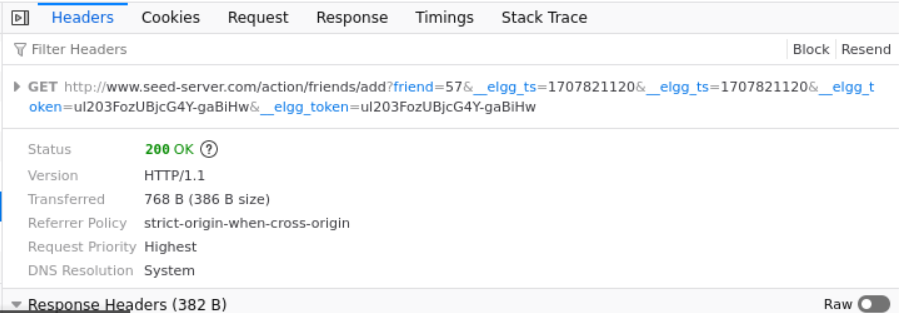
\includegraphics[width = 0.95\linewidth, center]{img/task1/1a.png}
    \caption{Task 1: Request Body}
    \label{fig:task1a}
\end{figure}
\begin{figure}[H]
    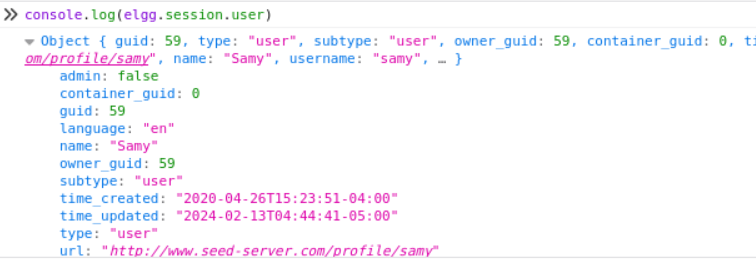
\includegraphics[width = 0.95\linewidth, center]{img/task1/1b.png}
    \caption{Task 1: \texttt{elgg.session.user} object}
    \label{fig:task1b}
\end{figure}
\begin{figure}[H]
    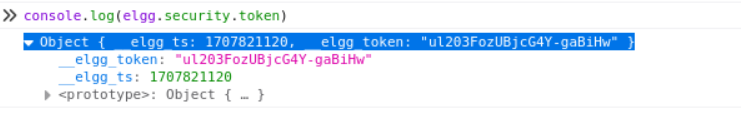
\includegraphics[width = 0.95\linewidth, center]{img/task1/1c.png}
    \caption{Task 1: \texttt{elgg.security.token} object}
    \label{fig:task1c}
\end{figure}
\begin{figure}[H]
    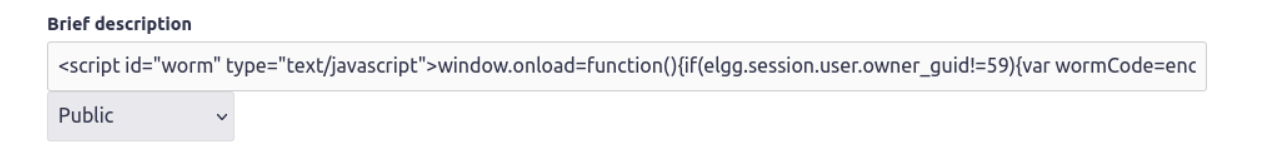
\includegraphics[width = 0.95\linewidth, center]{img/task1/1d.png}
    \caption{Task 1: Adding Script}
    \label{fig:task1d}
\end{figure}


\section{Task 2: Editing User's Profile}
\subsection{Method}
For this task, first the request for adding a user as a friend was inspected. The URL(\texttt{http://www.seed-server.com/action/profile/edit}), the request type(POST) and the query parameters was noted. A script was written that gets some of these values from the \texttt{elgg.session.user} and the \texttt{elgg.security.token} objects, sets other query parameters to random string, creates proper URL for editing a profile and sends a \texttt{XMLHttpRequest} to edit the user's profile. Samy's userid was hardcoded to ensure the script does not affect Samy himself. URL encoding was used to escape special characters in the URL. The script was added in the \textit{Brief Description} field of Samy's user profile so that it does not show in user preview.
\subsection{Screenshots}
\begin{figure}[H]
    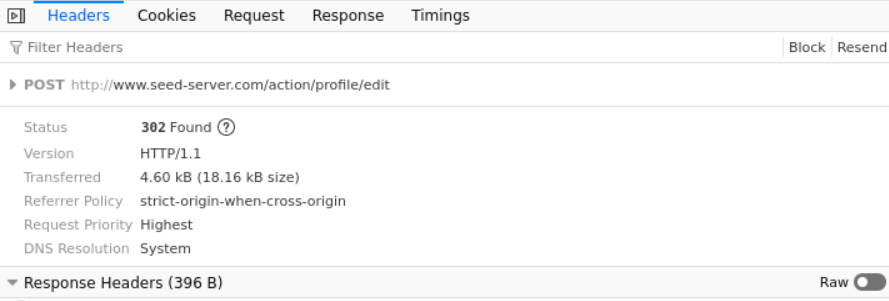
\includegraphics[width = 0.95\linewidth, center]{img/task2/2a.png}
    \caption{Task 2: Request Header}
    \label{fig:task2a}
\end{figure}
\begin{figure}[H]
    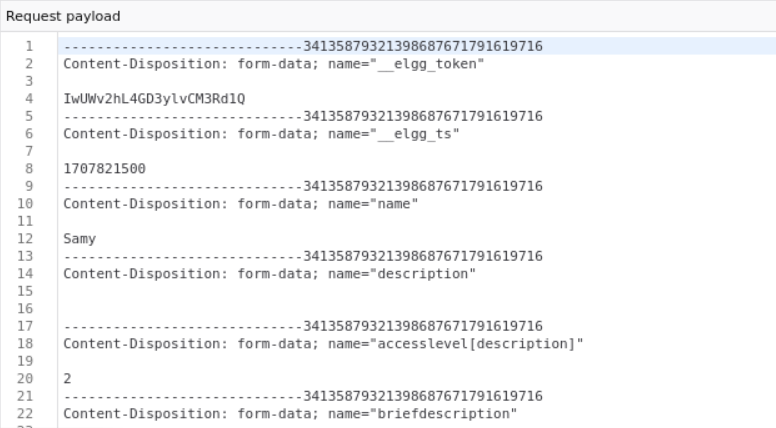
\includegraphics[width = 0.95\linewidth, center]{img/task2/2b.png}
    \caption{Task 2: Request Body}
    \label{fig:task2b}
\end{figure}
\begin{figure}[H]
    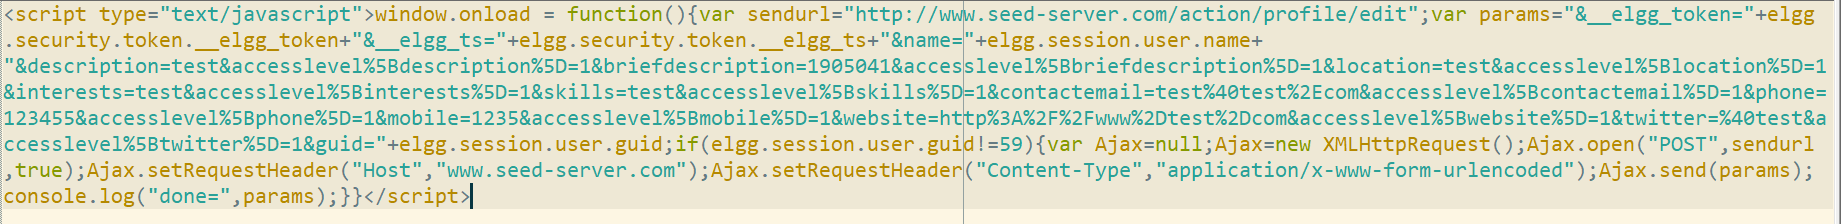
\includegraphics[width = 0.95\linewidth, center]{img/task2/2c.png}
    \caption{Task 2: URL encoded parameters, the script is dense due to character size limitations in input fields.}
    \label{fig:task2c}
\end{figure}

\section{Task 3: Posting On the Wire as User}
\subsection{Method}
For this task, first the request for posting on the wire was examined. The URL(\texttt{http://www.seed-server.com/action/thewire/add}), the request type(POST), the query parameters(\texttt{body, \_\_elgg\_token, \_\_elgg\_ts}) was noted. A script was written that gets these values from the \texttt{elgg.session.user} and the \texttt{elgg.security.token} objects, creates proper URL for posting on the wire and sends a \texttt{XMLHttpRequest} to post on the wire. Samy's userid was hardcoded to ensure the script does not affect Samy himself. URL encoding was used to escape special characters in the URL. The script was added in the \textit{Brief Description} field of Samy's user profile so that it does not show in user preview.
\subsection{Screenshots}
\begin{figure}[H]
    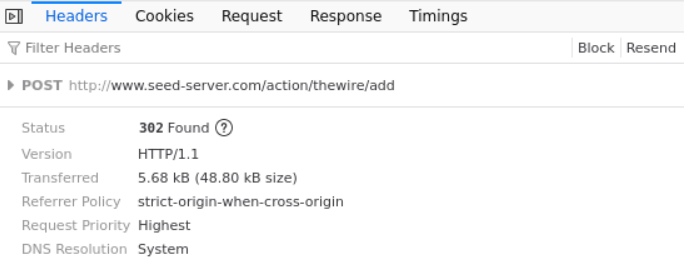
\includegraphics[width = 0.95\linewidth, center]{img/task3/3a.png}
    \caption{Task 3: Request Header}
    \label{fig:task3a}
\end{figure}
\begin{figure}[H]
    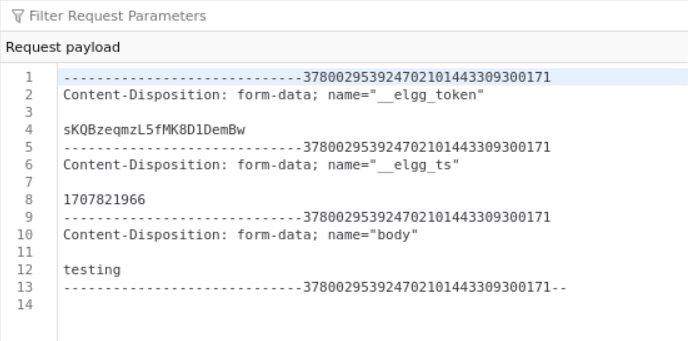
\includegraphics[width = 0.95\linewidth, center]{img/task3/3b.png}
    \caption{Task 3: Request Body}
    \label{fig:task3b}
\end{figure}

\section{Task 4: Self Propagating XSS Worm}
\subsection{Method}
For this task, code for task 1, 2 and 3 were combined. The script read it's own code using DOM and it's script id. The URL(\texttt{http://www.seed-server.com/action/friends/add?friend=59}), with request type(GET) and query parameters(\texttt{friend, \_\_elgg\_token, \_\_elgg\_ts}) was used to add Samy as a friend. \texttt{\_\_elgg\_token, \_\_elgg\_ts} values were accessed from the \texttt{elgg.session.user} and the \texttt{elgg.security.token} objects. The URL(\texttt{http://www.seed-server.com/action/profile/edit}) with request type(POST) and proper query parameters was used to add the worm in victim user's profile.  The URL(\texttt{http://www.seed-server.com/action/thewire/add}), the request type(POST), the query parameters(\texttt{body, \_\_elgg\_token, \_\_elgg\_ts}) was used to post the user's profile link on the wire. Samy's userid was hardcoded to ensure the script does not affect Samy himself.
\subsection{Screenshots}
\begin{figure}[H]
    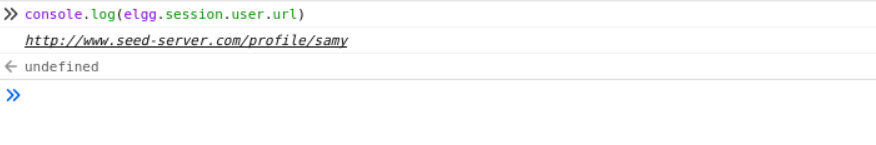
\includegraphics[width = 0.95\linewidth, center]{img/task4/4a.png}
    \caption{Task 4: Getting User URL}
    \label{fig:task4a}
\end{figure}
\begin{figure}[H]
    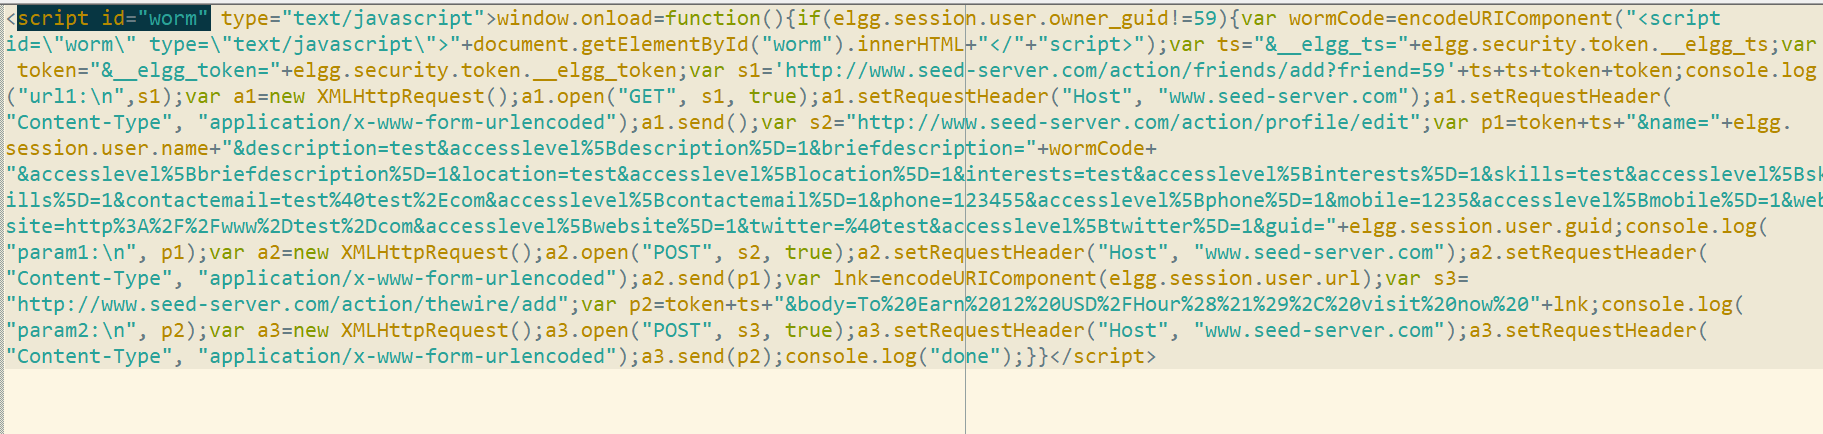
\includegraphics[width = 0.95\linewidth, center]{img/task4/4b.png}
    \caption{Task 4: Script id to access selfcode, the script is dense due to character size limitations in input fields}
    \label{fig:task4b}
\end{figure}

\end{document}+++---